% !Mode:: "TeX:UTF-8"
% !TEX program  = xelatex
\section{Analysis of model structure and parameter setting}
\subsection{Performance of Autoencoder, VAE and ZIVA}
Our model was adapted from the variational autoencoder (VAE). The major improvement is the zero-inflation layer. So, I analyzed the significance of the ZI layer in this part. I performed the Autoencoder, Variational autoencoder, and ZIVA to several data and evaluated their performance on visualization and clustering. We performed visualization (Figure \ref{3ae}) and clustering (Table \ref{t3ae}, Figure \ref{3aeclu}) to the dimensionality reduction results under two dimensions. Both the visualization and the clustering evaluation show that ZIVA performs better than autoencoder and variational autoencoder. It is proven that the zero-inflation layer works in our network structure. \\
\begin{figure}[htb!]
    \centering
    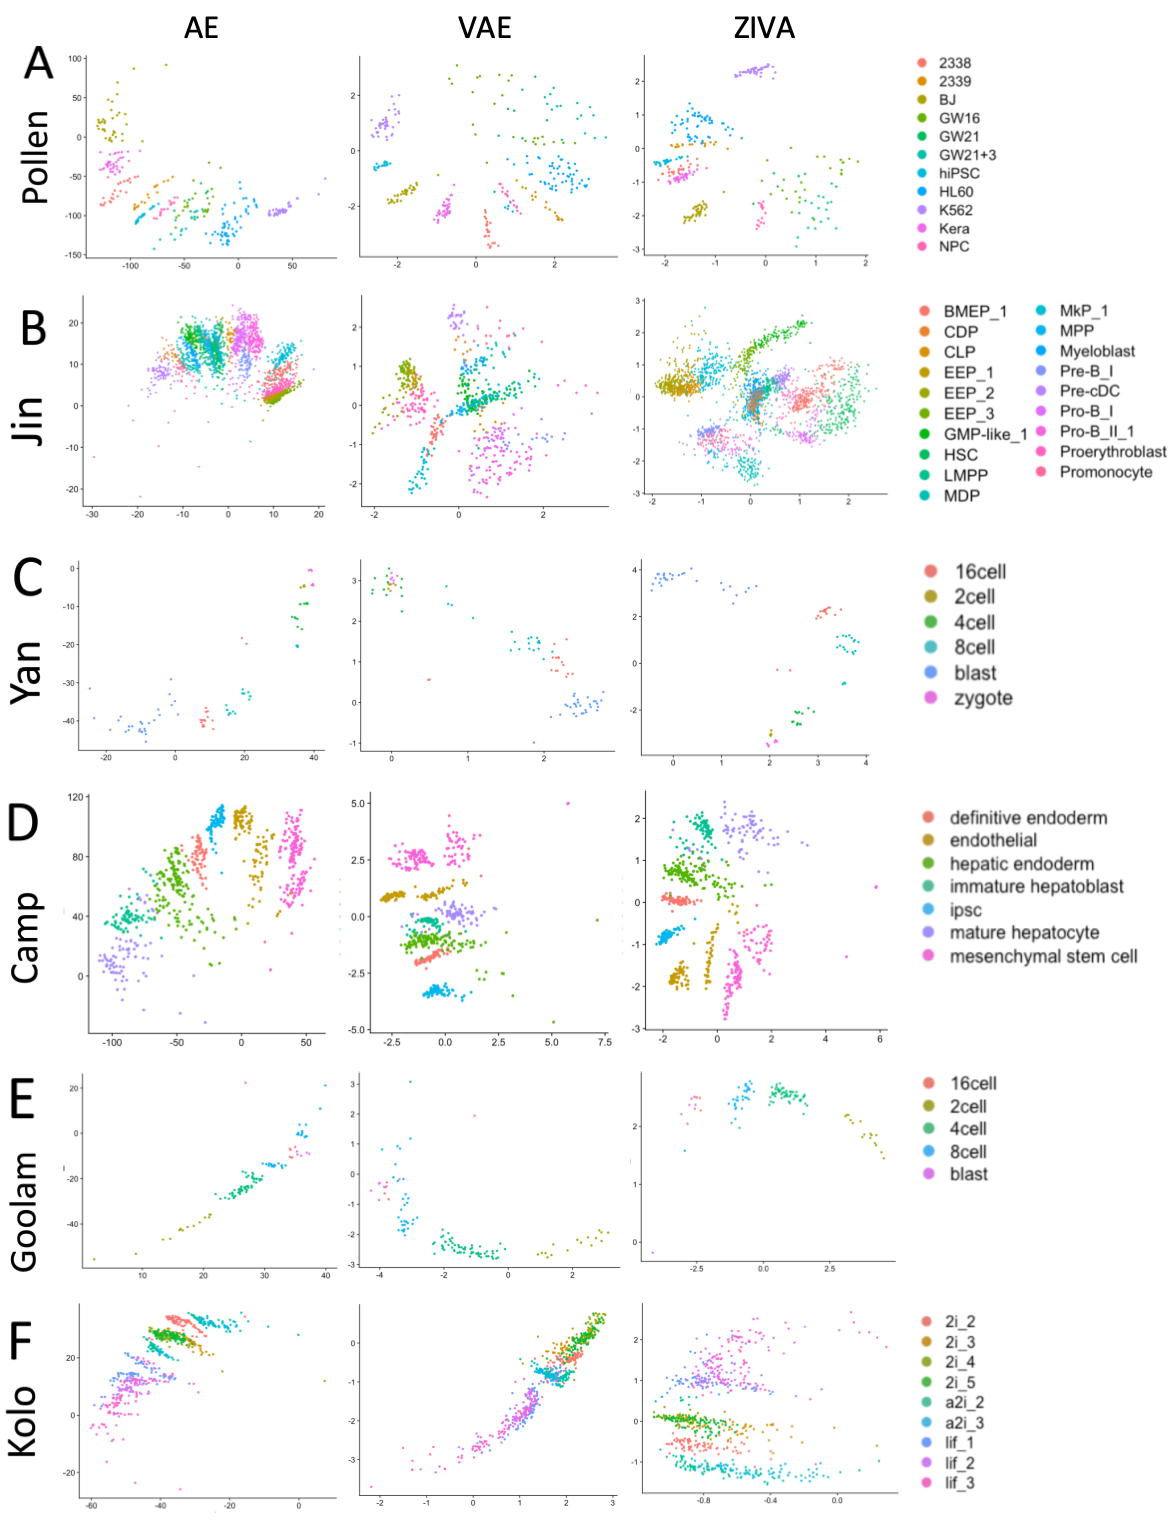
\includegraphics[width=0.8\textwidth]{figures/myfigures/3ae.png}
    \caption{Visualization of scRNA-seq datasets using Autoencoder, Variational autoencoder (VAE) and ZIVA}
    \label{3ae}
\end{figure}

\begin{figure}[htb!]
    \centering
    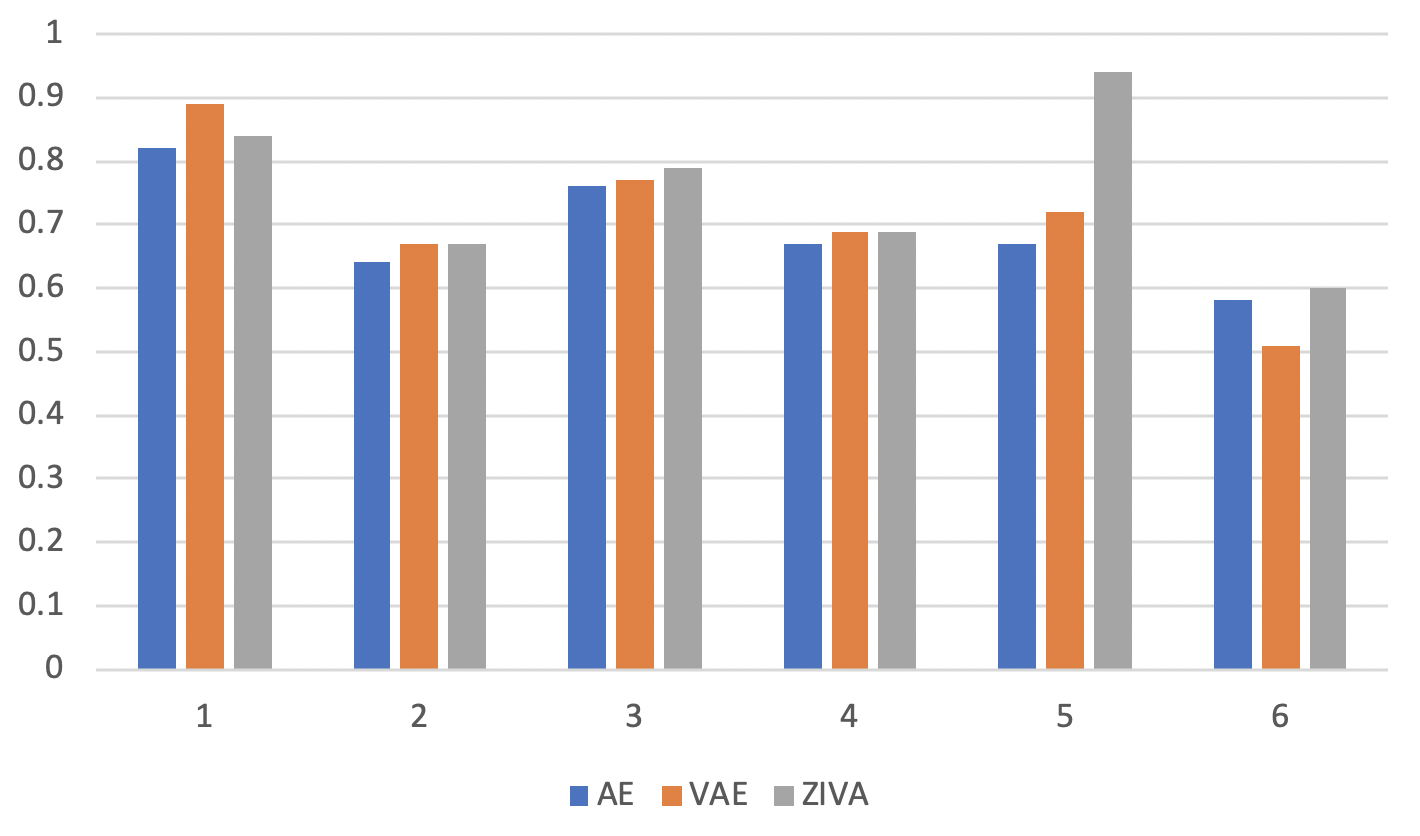
\includegraphics[width=0.8\textwidth]{figures/myfigures/3aeclu.png}
    \caption{Clustering performance comparation among Autoencoder, Variational autoencoder (VAE) and ZIVA}
    \label{3aeclu}
\end{figure}

\begin{table}[htb!]
\centering
\caption{NMI and ARI of clustering performance of Autoencoder, VAE and ZIVA.}
\label{t3ae}
\begin{tabular}{lllllll}
\hline
  & \multicolumn{3}{l}{NMI} & \multicolumn{3}{l}{ARI} \\ \hline
  & AE     & VAE    & ZIVA  & AE     & VAE    & ZIVA  \\ \hline
1 & 0.82   & 0.89   & 0.84  & 0.73   & 0.87   & 0.75  \\
2 & 0.64   & 0.67   & 0.67  & 0.37   & 0.41   & 0.43  \\
3 & 0.76   & 0.77   & 0.79  & 0.63   & 0.74   & 0.64  \\
4 & 0.67   & 0.69   & 0.69  & 0.48   & 0.52   & 0.51  \\
5 & 0.67   & 0.72   & 0.94  & 0.72   & 0.54   & 0.98  \\
6 & 0.58   & 0.51   & 0.60  & 0.40   & 0.33   & 0.43  \\ \hline
\end{tabular}
\end{table}

\clearpage

\subsection{Analysis of dropout model}
We then tested the performance of two dropout models: the double exponential model and the Michaelis-Menten model. We tested the performance of clustering on the data reduced to two dimensions by two methods. The result (Figure \ref{nbmmari}, Table \ref{tnbmm}) shows that two models have similar performance on those datasets.
\begin{figure}[htb!]
    \centering
    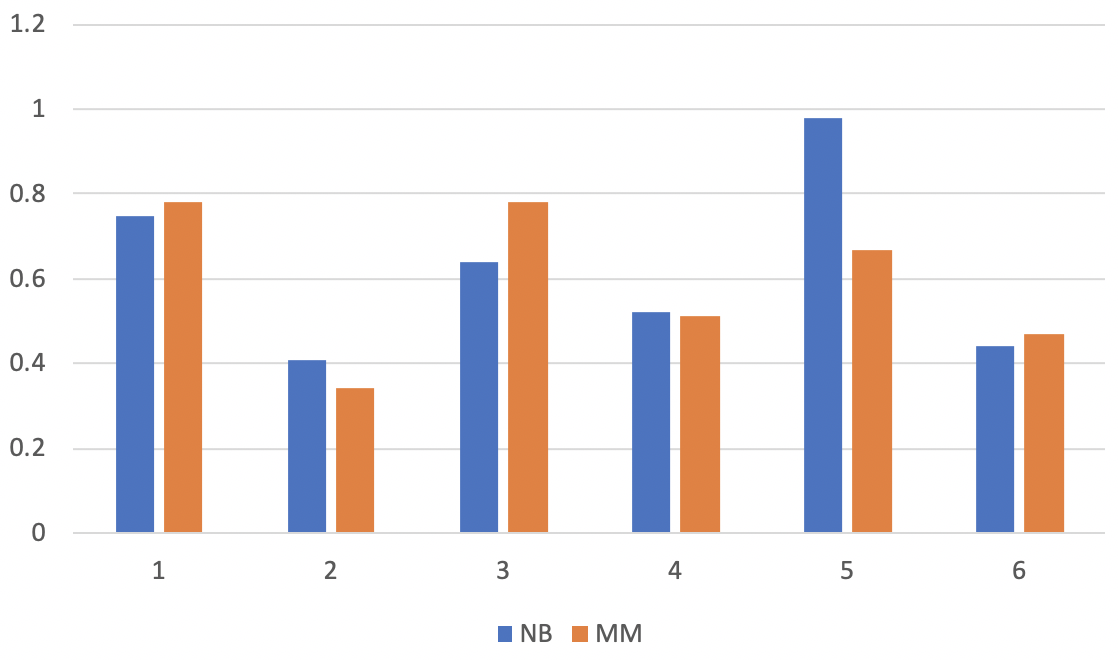
\includegraphics[width=0.8\textwidth]{figures/myfigures/nbmmari.png}
    \caption{Clustering performance (NMI and ARI) of ZIVA under different dropout models.}
    \label{nbmmari}
\end{figure}

\begin{table}[htb!]
\centering
\caption{NMI and ARI of clustering performance of ZIVA under different dropout model.}
\label{tnbmm}
\begin{tabular}{lllll}
\hline
  & \multicolumn{2}{l}{NMI} & \multicolumn{2}{l}{ARI} \\ \hline
  & DE         & MM         & DE         & MM         \\ \hline
1 & 0.84       & 0.84       & 0.75       & 0.78       \\
2 & 0.67       & 0.63       & 0.41       & 0.34       \\
3 & 0.79       & 0.87       & 0.64       & 0.78       \\
4 & 0.69       & 0.68       & 0.52       & 0.51       \\
5 & 0.94       & 0.83       & 0.98       & 0.67       \\
6 & 0.61       & 0.64       & 0.44       & 0.47       \\ \hline
\end{tabular}
\end{table}

\clearpage

\subsection{Analysis of the function of the nuclear norm}
When designing the model, we added the third part to the original VAE loss function, which is the rank of the output matrix from decoder $\widetilde{\boldsymbol{Y}}$. Because there are only a limited number of cell types and the expression matrix is extremely sparse, we assume that the data matrix should have a low rank. However, the rank of a matrix is hard to computed and is not convex. Nuclear norm \cite{Zhang_2010} was used to approximate the rank. The nuclear norm is also called trace norm, is a convex approximation of the rank. It means the summation of the singular values of a matrix. It is a suitable choice for loss function because it is convex and differentiable. In this way, the recovered matrix's rank should be as small as possible because there are only a limited number of distinct cell types.

Here, we test the effect of the nuclear norm. We chose the weight of the nuclear norm to be 0, 0.0001, 0.001, 0.01, and 0.05 to test its performance. The results are shown in Figure \cite{nuclear}. The effect of the nuclear norm is not good and has some harmful effects. Because the inputted expression matrix has many noises and thus does not have the property of low rank, in this case, if we add such regularization to the output matrix, it will render the effect of the whole model. It shows that the nuclear norm here is not suitable. Therefore, we finally removed this part in our model structure.

\begin{figure}[htb!]
    \centering
    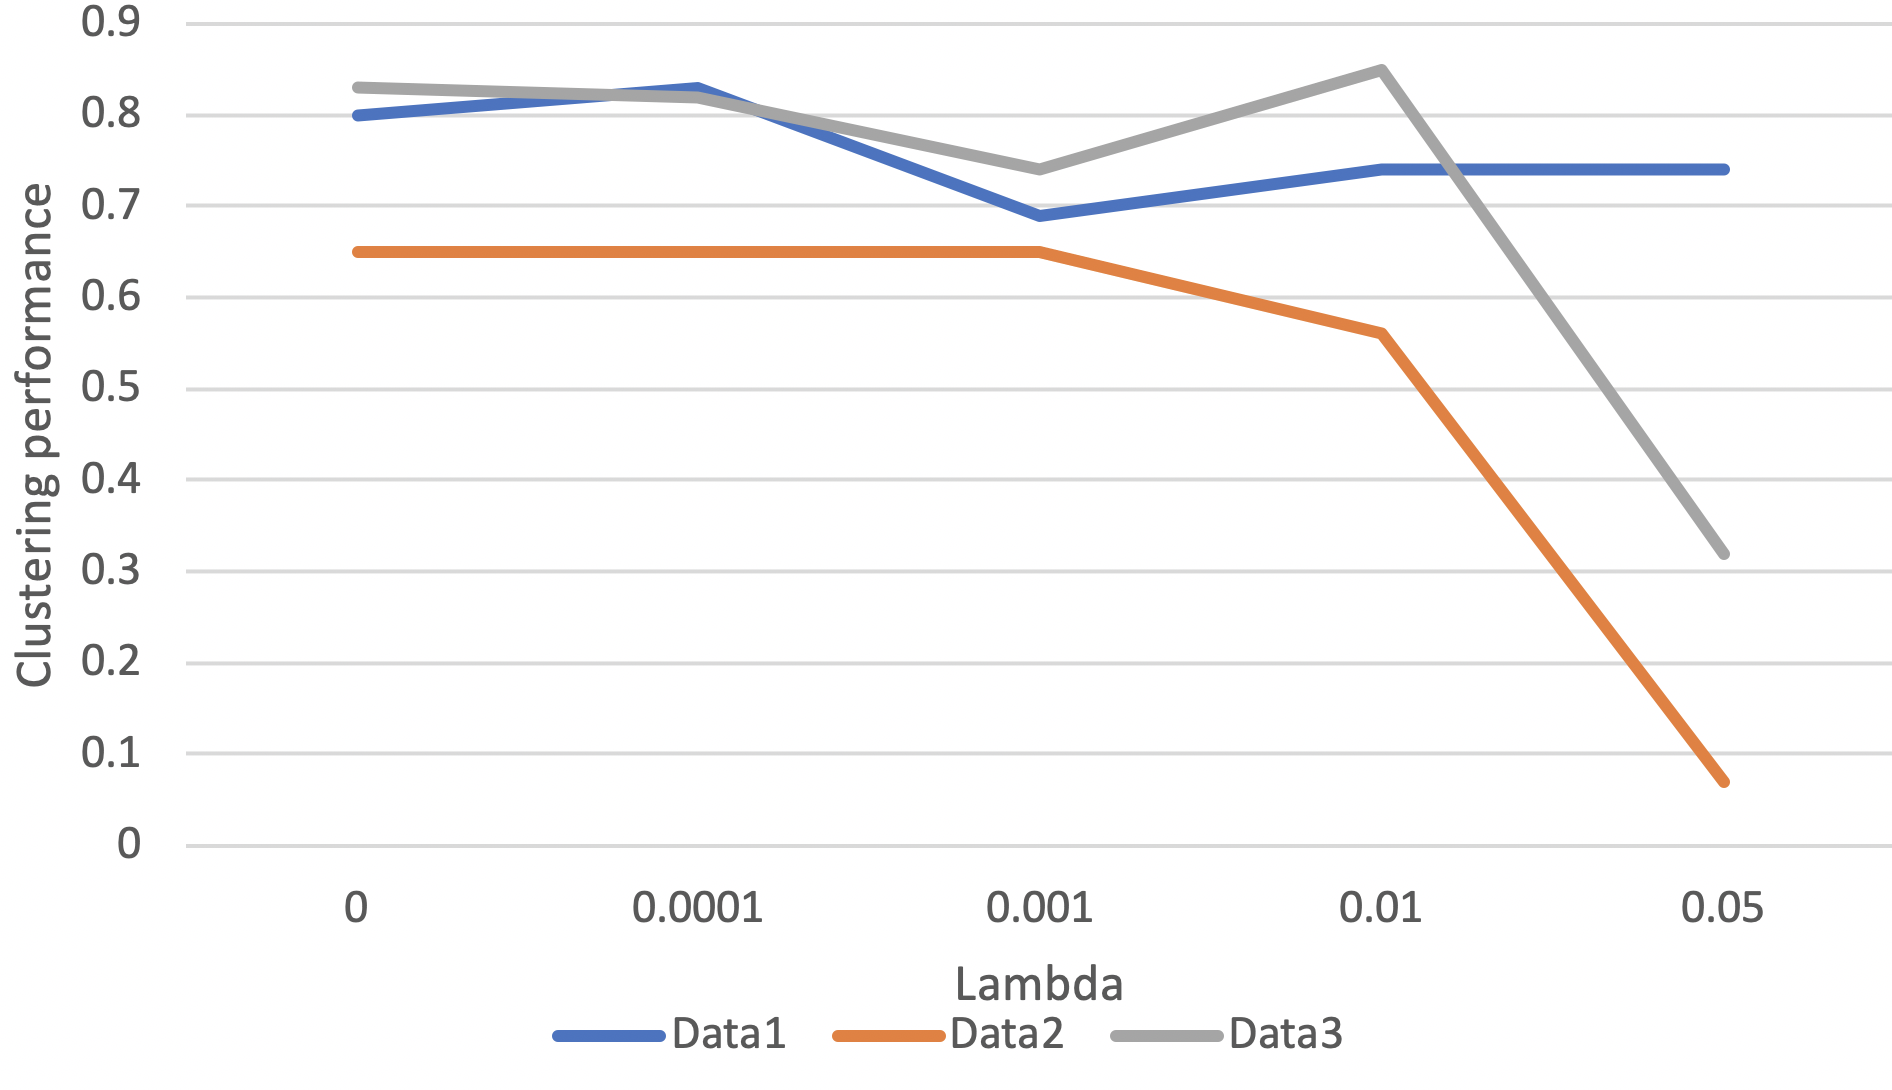
\includegraphics[width=0.8\textwidth]{figures/myfigures/nuclear.png}
    \caption{Clustering performance (NMI and ARI) of ZIVA using different weight of nuclear norm.}
    \label{nuclear}
\end{figure}

\clearpage

\subsection{Analysis of latent dimensions}
I then tested the clustering performance under different latent dimensions (2, 4, 6, 8, 10, 15, 20, all). The result (Table \ref{dimt}, Figure \ref{dim}) shows that there is no significance difference among different latent dimensions. The performance on two dimensions and all dimensions are slightly higher. According to this result, the first two dimensions are enough for downstream analysis. That suggests that the data of scRNA-seq is extremely sparse.
\begin{figure}[htb!]
    \centering
    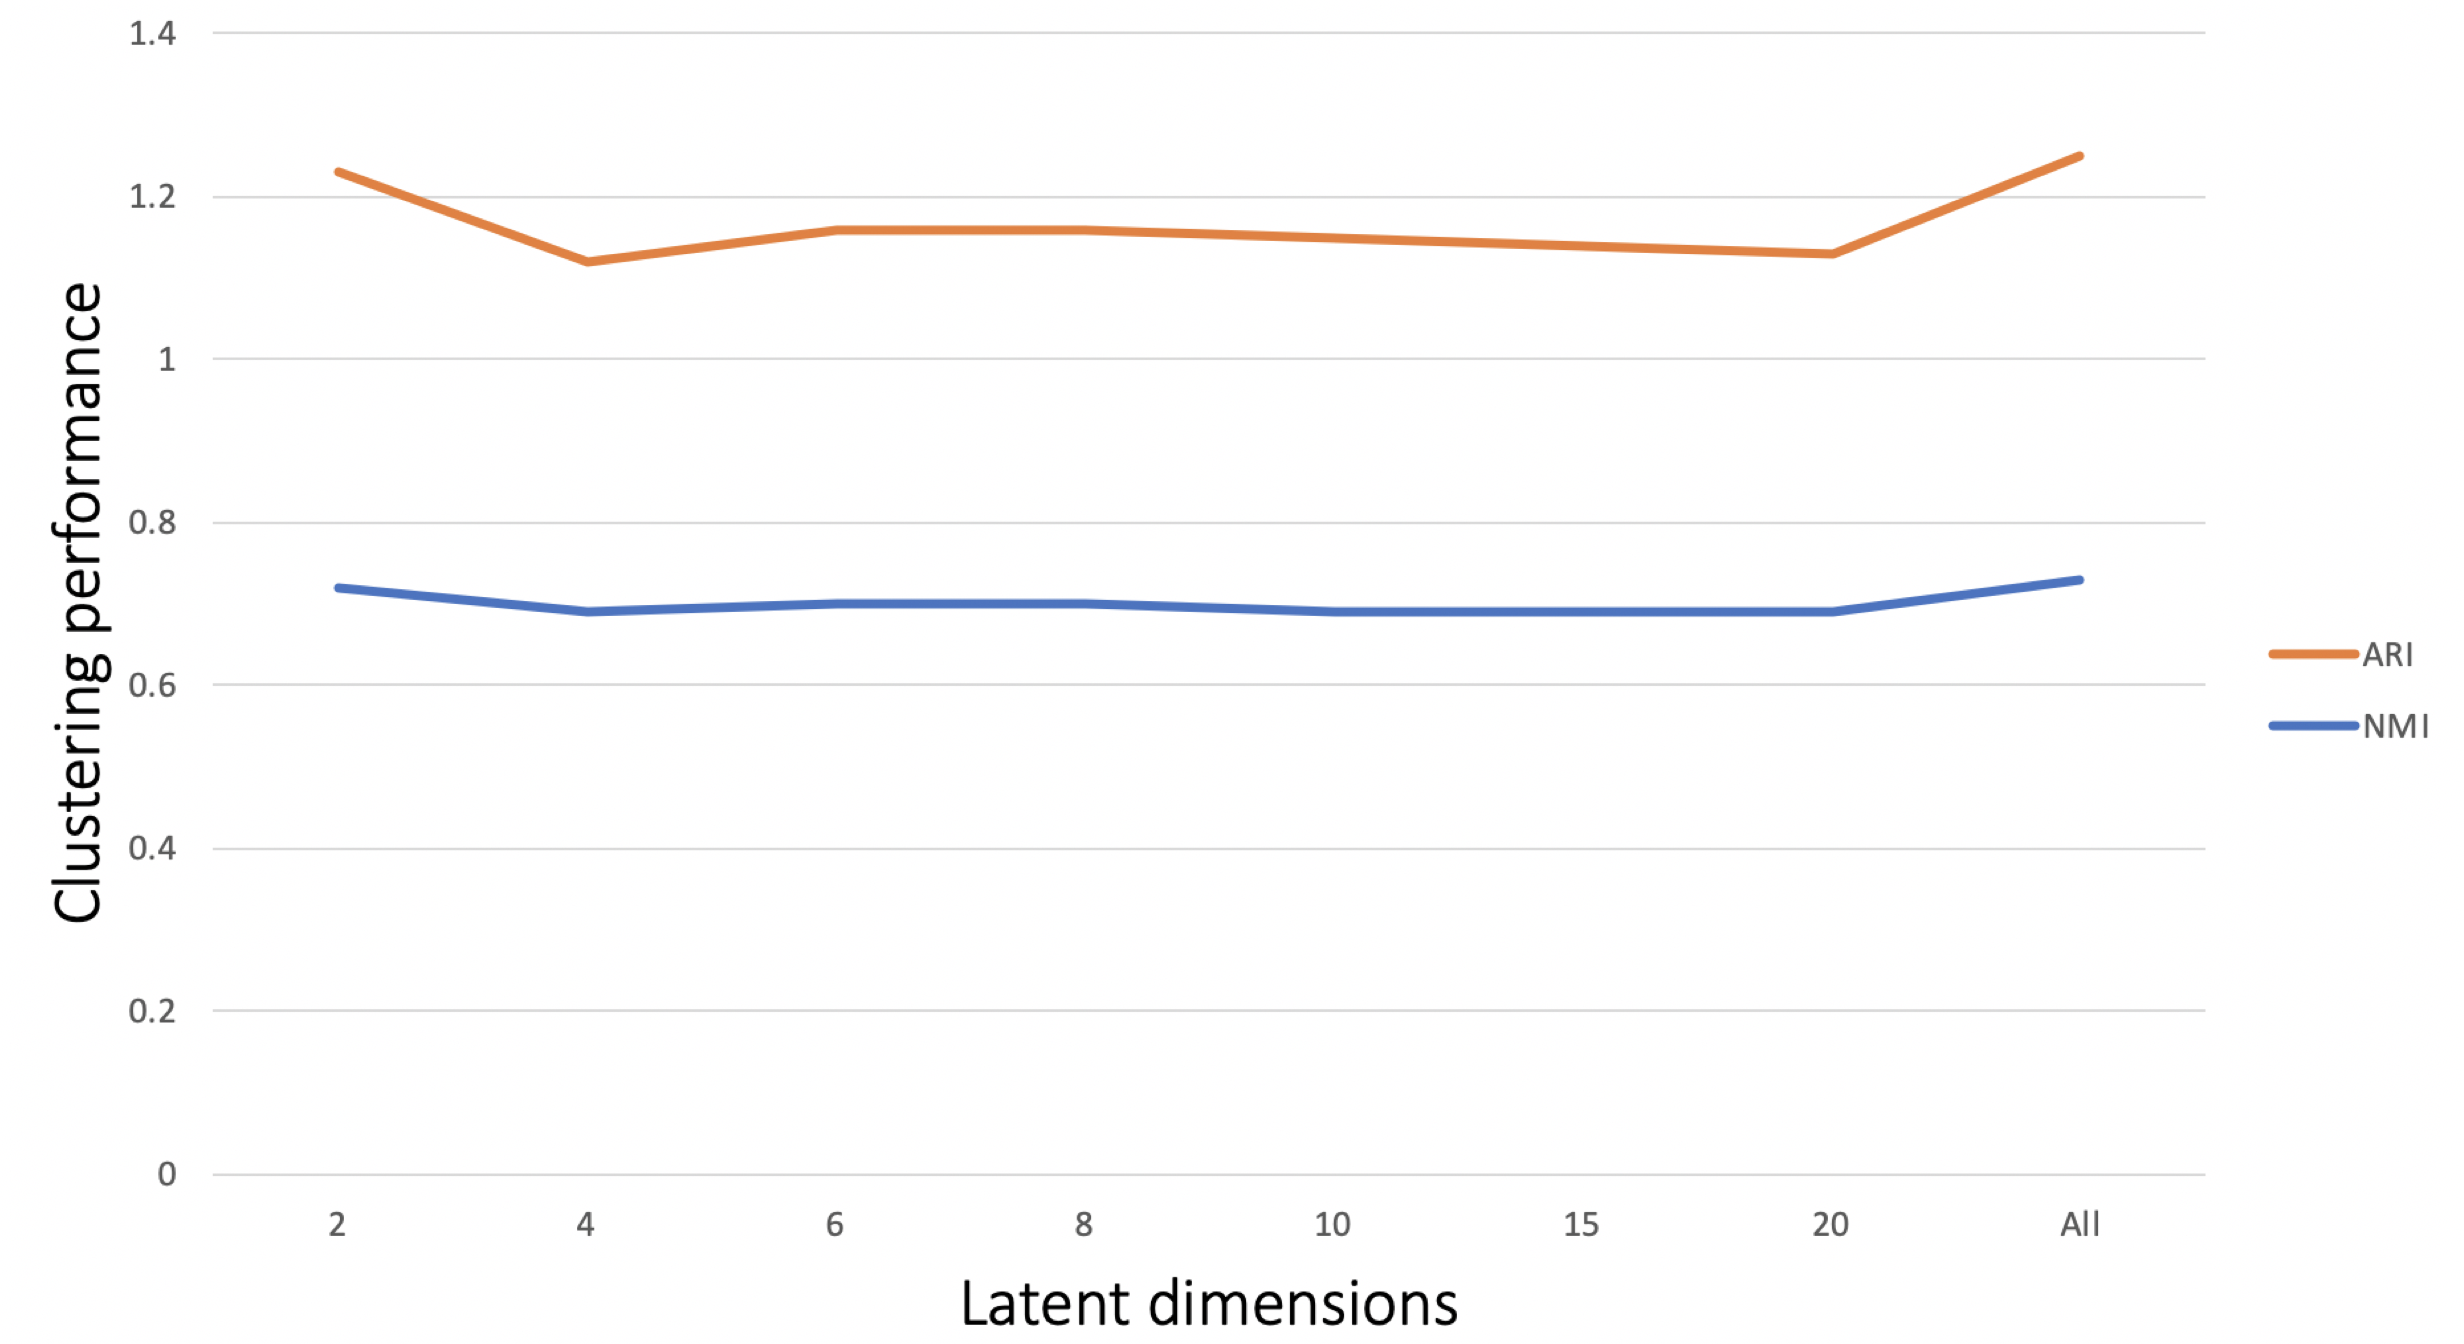
\includegraphics[width=0.8\textwidth]{figures/myfigures/dim.png}
    \caption{Clustering performance (NMI and ARI) of ZIVA under different latent dimensions.}
    \label{dim}
\end{figure}

\begin{table}[htb!]
\centering
\caption{NMI and ARI of clustering performance of ZIVA under different latent dimensions.}
\label{dimt}
\begin{tabular}{lllllllll}
\hline
    & 2    & 4    & 6    & 8    & 10   & 15   & 20   & All  \\ \hline
NMI & 0.72 & 0.69 & 0.70 & 0.70 & 0.69 & 0.69 & 0.69 & 0.73 \\
ARI & 0.51 & 0.43 & 0.46 & 0.46 & 0.46 & 0.45 & 0.44 & 0.52 \\ \hline
\end{tabular}
\end{table}